\documentclass[11pt]{article}
\usepackage[margin=1.1in]{geometry}
\usepackage{amsmath,amssymb,amsthm}
\usepackage{booktabs}
\usepackage{array}
\usepackage{tabularx}
\usepackage[protrusion=true,expansion=false]{microtype}
\usepackage[table]{xcolor}
\usepackage{enumitem}
\usepackage{titlesec}
\usepackage{tikz}
\usepackage{float}
\usetikzlibrary{arrows.meta,positioning,fit,calc,decorations.pathreplacing}
\usepackage{listings}
\usepackage{hyperref}

\hypersetup{colorlinks=true, linkcolor=blue!60!black, urlcolor=blue!60!black, citecolor=blue!60!black}
\usepackage[skip=0.6\baselineskip, indent=0pt]{parskip}

\titleformat{\section}{\large\bfseries}{\thesection.}{0.7em}{}
\titleformat{\subsection}{\normalsize\bfseries}{\thesubsection.}{0.6em}{}

\newcommand{\vmax}{V_{\max}}
\newcommand{\Tc}{T_{\mathrm{close}}}
\newcommand{\tx}[1]{\texttt{#1}}
\newcolumntype{L}{>{\raggedright\arraybackslash}X}

\lstdefinestyle{script}{
  basicstyle=\ttfamily\small,
  columns=fullflexible,
  keepspaces=true,
  breaklines=true,
  frame=single,
  framerule=0.3pt,
  xleftmargin=1em,
  escapeinside={(*}{*)},
}

\newtheorem{assumption}{Assumption}

% tables: a little more room between rows, and every other row shaded, so
% that rows of wrapped text stay distinct
\renewcommand{\arraystretch}{1.3}
\rowcolors{1}{}{black!5}

\definecolor{coop}{RGB}{232,245,233}
\definecolor{chainc}{RGB}{255,228,225}
\definecolor{proofc}{RGB}{230,240,255}

\title{\textbf{Lichen}\\L2s In CHannels ENforced by bitcoin}
\author{waxwing}
\date{Version 0.4, October 2026}

\begin{document}
\maketitle

\begin{abstract}
A \emph{contract} with a hub lets a user hold the hub's tokens on a layer 2 and
withdraw them as bitcoin without trusting the hub for honesty or liveness. The L2 tokens are collateralised by the bitcoin in the user-hub multisig output\footnote{a standalone 2-of-2 output (a channel embedding is possible; Section~\ref{sec:contract})}, and if the hub refuses a withdrawal, or cannot answer because it is offline, it is enforced on Bitcoin. The only assumptions are those of the layer 2 itself. \underline{No change to Bitcoin's
consensus is required}. A withdrawal is a claim that a program, the withdrawal statement, ran on some input and produced an output: the statement is proved with RISC Zero and wrapped in Groth16, and a disputed claim is settled on Bitcoin by a \emph{verification gadget} that checks the Groth16 proof: the one chosen is BABE~\cite{babe}, using witness encryption and garbled circuits, in four or five transactions (BitVMX~\cite{bitvmx} is also implemented and tested).  Withdrawals are executed cooperatively in the contract --- the normal case, because the statement is deterministically verifiable in milliseconds --- or, otherwise, a refused one is played as a dispute on chain, set up at the start of each contract. The trustlessness gain is paid for with liquidity (with receiving ability only contingent on offered ``inbound'' from the hub, as in Lightning). The hub (but not user) must also stay live during normal operation, since an offline hub loses disputes by timeout. The design, including an example privacy-focused, shielded note style L2, is built and measured in~\cite{lichencode}.
\end{abstract}

\tableofcontents

%\section{Introduction}

\section{Obvious objections to Lichen and why they're mostly wrong}

\paragraph{One central hub is dangerous.} If the hub disappears, the user gets the money. The hub cannot Sybil attack users by printing tokens fictitiously; the honest users' money is all backed. The only remaining risks are inherent to the L2 itself (is it a validity rollup or a quorum? Does it inherit finality from Bitcoin or is finality weaker? Etc.)

\paragraph{Bridges usually mean you can only withdraw a fixed size utxo, meaning operators and relying on swaps. Surely that applies here?} No. The withdrawal amount is encoded in bits in the bitcoin transaction witness, in dispute. This allows us to withdraw arbitrary amounts via multiple outputs of certain denominations~[\ref{sec:outcomes}].

\paragraph{Don't these constructions usually require a 1 of n honesty assumption from a signing committee?} Not here: we avoid this by the LN-GAP~\cite{lngap} trick: the contract is a \emph{bilateral} contract between the hub and each user; the presigning happens between them, just as in Lightning.

\paragraph{But if a bunch of users open contracts with a hub, they can just .. pay each other through Lightning channels?} A correct critique, partly, \underline{if} the L2 ledger doesn't do anything but plain payments. Even then, you could avoid receiver liveness being needed, avoid routing and other minor things. But the real answer is: the L2 can offer more functionality. It can offer private payments, smart contracts, etc.

\paragraph{But this is an IOU/ hub's token, so it's not actually bitcoin.} Incorrect with a crucial caveat. See the first point: every sat is redeemable via the user-hub contracts, \emph{without} the hub's permission, via the contract utxo, so these are actually bitcoin \emph{but only as long as you have liquidity to receive them}. A new user on L2 without a contract with the hub, or a user holding a balance on L2 in excess of their inbound liquidity in their own contract, is holding \emph{credit}, and has no such guarantee. But that's their choice.

\paragraph{But still, a single central hub feels like bad design. Why not multiple hubs?} Having multiple hubs \emph{will} make sense --- see Section~\ref{sec:multihub}, but done naively, it is broken. It's because of what these L2 tokens are. They are fungible, \underline{enforceable} claims on the hub's money; they are minted by the hub itself, just on its own say-so. If you had hub 1 and hub 2, those claims are not transferrable trustlessly to the hubs themselves. If hub 2 prints a billion sats out of nothing and users accept it on the L2 they can redeem it with hub1, leaving hub1 out of pocket. From this line of thinking we see an interesting comparison with ecash servers: the hub can print as much as it likes, but it cannot steal/``rug''.

\paragraph{So what's the catch?} The negatives are twofold: one is liquidity, and this is easy to understand as the analog of the inbound liquidity pain point in Lightning, because it's basically the same thing. Such a hub \emph{can} choose to give no inbound liquidity to a user: they get tokens on L2 to spend, but they cannot (safely) receive. If they receive, it's just credit that someone else will hopefully buy from them. But the design does not assume that, of course, it allows receiving up to a ``cap'': the user negotiates that extra potential receiving amount (inbound liquidity) when it sets up the contract with the hub. The second is the on-chain dispute, whose size depends on the gadget: four or five transactions and 10--31~kvB under BABE, lichen's gadget, against tens of transactions and 100--200~kvB under BitVMX, the first, both as measured on Mutinynet~\cite{lichenbuilt,lichenbitvmx}.

%\subsection{A note on the delta to LN-GAP}
%\label{sec:family}

%LN-GAP~\cite{lngap} puts contracts governed by arbitrary programs into Lightning~\cite{lightning}
%channels: a contract's outcome is decided by a game whose moves are
%signed off-chain, with pre-signed transactions that let either party
%take a dispute to Bitcoin~\cite{lngap}. Lichen mainly differs in trying to achieve trustlessness at the expense of a potentially larger (though still O(1) in the size of the withdrawal statement) onchain resolution; a tradeoff that fits well with the intent of creating \emph{an L2 from a bunch of contracts with a hub}:

%\begin{center}
%\small
%\begin{tabularx}{\linewidth}{p{24mm}LL}
%\toprule
%& LN-GAP &  Lichen w/ BABE  \\
%\midrule
%venue & trusted: a majority of members attests moves & none \\
%a dispute is decided by & the venue's attestations  & the chain: a challenge, answered from garbled circuits \\
%suited to & interactive games where time has value  & withdrawals from a hub's layer 2 \\
%on-chain cost of a dispute & constant & constant: about 30~kvB \\
%\bottomrule
%\end{tabularx}
%\end{center}

%\paragraph{Why Lichen needs no venue.}  It's more about choice than logical requirement. In LN-GAP the parties \emph{could} just play ForceMove and accept that the game goes onchain when someone is not cooperative. That's not much fun for a 100 move chess game or similar. However the tradeoff of trust vs length of game is drastically different for Lichen: the game length is fixed in advance, and with BABE it is short: four or five transactions. While for such an L2 to be viable it's absolutely crucial to try to remove third party trust. That's why the ``venue'' concept is removed here.

\section{Contracts with the hub}
\label{sec:terms}

\textbf{Alice}, the user, has a contract with a \textbf{Hub}, instantiated as a 2 of 2 output  (see Section~\ref{sec:contract} for the possibility of embedding this inside a Lightning channel), with these terms:
\begin{center}
\small
\begin{tabularx}{\linewidth}{p{16mm}L}
\toprule
$D$ & Alice's deposit: she puts $D$ bitcoin in and receives $D$ of the hub's tokens on the L2 \\
$\vmax$ & the most she can withdraw: her $D$ plus the hub's liquidity $\vmax - D$ (which can be zero)\\
$r_A, r_H$ & the \emph{contract reserves}, for fees. Forfeited by losing side of a dispute, otherwise returned to owner. (Section~\ref{sec:outcomes}); the contract holds $\vmax + r_A + r_H$ \\
$b$ & the amount she withdraws, by returning $b$ tokens to the hub on the L2 with the memo $c$ \\
$c$ & the contract's identifier, its memo \\
$\Tc$ & the contract's end: with no withdrawal by then, the hub takes it \\
\bottomrule
\end{tabularx}
\end{center}
Every token is a liability of the hub, collateralised by the contract of whoever holds it, within that holder's cap; within $\vmax$ and before $\Tc$, Alice trusts the hub for nothing, not even to be online: a withdrawal it does not answer is paid by timeout.

\paragraph{Opening is atomic.} Alice's $D$ goes into the contract and this entitles her
$D$ tokens on the L2. This must be atomic: a hub
that took the funding and never minted would leave her nothing to
return, and the default at $\Tc$ would hand it her $D$; a hub that
minted first could be left with tokens backed by no contract. Alice
first pays a deposit output\footnote{A well known design pattern to avoid the need for Alice's external wallet to support some kind of co-signing event}, the hub's key and hers together, or hers
alone after a timeout. The hub then mints $D$ to the key
$P = H(A \,\|\, T)\cdot A + T$, where $A$ is Alice's L2 key and $T = t\cdot G$
a point of the funding transaction's own (the coefficient keeps Alice
from choosing $A$ against $T$), and Alice, once she sees that mint
final on L2, signs the funding's deposit input as an adaptor pre-signature
locked to $T$. The hub can lock the deposit only by completing the adaptor,
which publishes $t$ and so unlocks her tokens. The hub's side needs no
refund: if it never broadcasts, Alice refunds the deposit, and the
locked tokens, which cost nothing to print, stay where they are. Its one
risk is timing: $t$ is public once the funding is in the mempool, so it
broadcasts only well before the deposit's refund matures.

\begin{figure}[H]
\centering
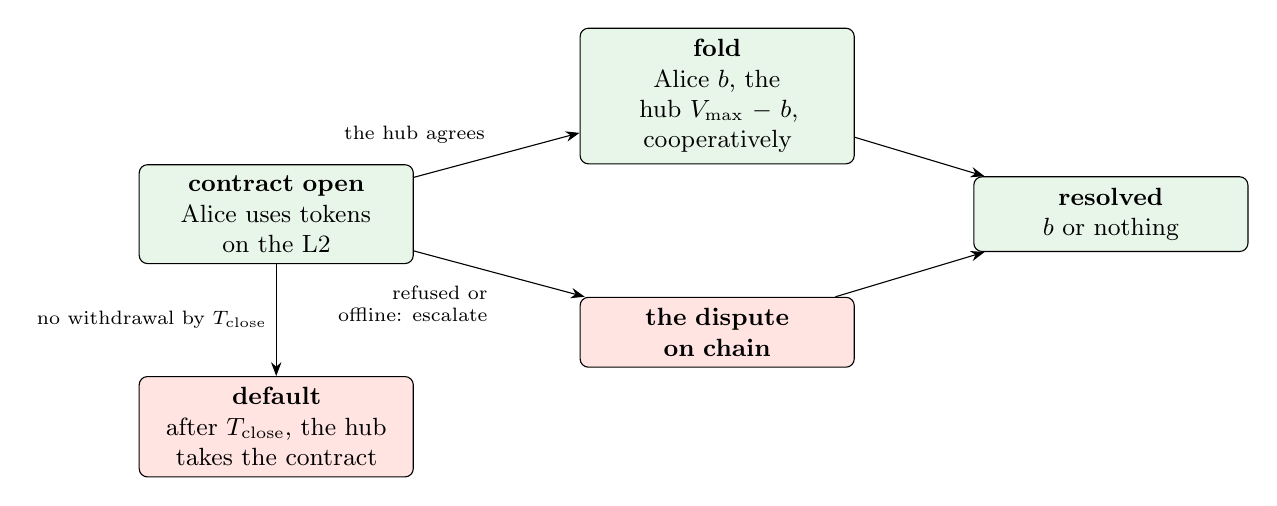
\begin{tikzpicture}[
  font=\small,
  st/.style={draw, rounded corners=3pt, align=center, inner sep=4pt, text width=#1},
  st/.default=32mm,
  >={Stealth[length=5pt]},
]
\node[st, fill=coop] (live) at (0,0) {\textbf{contract open}\\Alice uses tokens\\on the L2};
\node[st, fill=coop] (fold) at (5.6,1.5) {\textbf{fold}\\Alice $b$, the hub $\vmax - b$,\\cooperatively};
\node[st, fill=chainc] (ladder) at (5.6,-1.5) {\textbf{the dispute on chain}};
\node[st, fill=chainc] (def) at (0,-2.7) {\textbf{default}\\after $\Tc$, the hub\\takes the contract};
\node[st, fill=coop] (end) at (10.6,0) {\textbf{resolved}\\$b$ or nothing};
\draw[->] (live) -- node[above left=1pt, font=\scriptsize] {the hub agrees} (fold);
\draw[->] (live) -- node[below left=1pt, font=\scriptsize, align=right] {refused or\\offline: escalate} (ladder);
\draw[->] (live) -- node[left, font=\scriptsize] {no withdrawal by $\Tc$} (def);
\draw[->] (fold) -- (end);
\draw[->] (ladder) -- (end);
\end{tikzpicture}
\caption{The life of a contract. Green states settle
cooperatively (and could remain offchain in channels).}
\label{fig:life}
\end{figure}

\section{How a withdrawal from the L2 is proved valid}
\label{sec:statement}

\subsection{The statement proved}

The details of the statement proved will of course depend on the L2's architecture. In abstract, the withdrawal request must be accompanied by a satisfaction of the predicate:

\[\mathcal{R}_L(\mathcal{D}, c, \ldots ; w=(b, \ldots))\]

where $\mathcal{D}$ is the deployment context (the settings of the L2), $c$ is the contract in Lichen between hub and user, $b$ is the amount in satoshis of withdrawal claimed, and $w$ is the secret witness used by the user to satisfy the predicate.

\paragraph{A note on secret inputs and public inputs.} Some parts of $w$ may not actually be secrets. Here we specifically include the withdrawal amount $b$; a peculiarity of our chosen verification gadget BABE is that practical usage of it requires a cut-and-choose setup that fixes the public input at contract setup; thus including any later-defined data must necessarily be in $w$. The mechanism to make this work is described in~\cite[\S 5]{lichenbuilt}.


Our verification gadget will verify a proof of satisfaction (specifically a Groth16 proof string) of this predicate.

 Let's take the simplest conceivable example, a single signing entity in full control of the L2. In that case, $w$ will include a signature by the signer, of the current state, and an inclusion proof of a withdrawal transaction/note whose value is $b$.
 
In more realistically interesting cases, for example:

\begin{itemize}
\item An L2 managed by a large quorum with threshold signing of some form
\item an L2 hosted on another blockchain such as Ethereum
\item an L2 using a single use seal on Bitcoin itself to achieve finality and validity proofs of state transition (such as our own design described in~\cite{lichenbuilt})
\end{itemize}

\ldots the degree to which trustless exit can be claimed will vary, but that is a matter for the L2 architecture: \underline{lichen simply enforces the L2's ruleset, and that part \emph{is} trustless}.

In the remainder of Section 3, we will focus on the mechanical details by which this is achieved.

\subsection{From a program to a verifiable claim}

\begin{figure}[H]
\centering
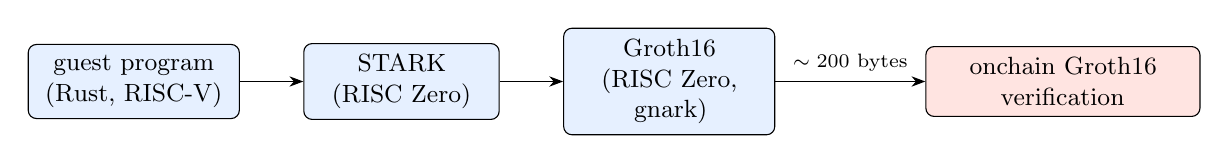
\begin{tikzpicture}[
  font=\small,
  box/.style={draw, rounded corners=3pt, align=center, inner sep=4pt, text width=#1},
  box/.default=27mm,
  >={Stealth[length=5pt]},
]
\node[box=24mm, fill=proofc] (g) at (0,0) {guest program\\(Rust, RISC-V)};
\node[box=22mm, fill=proofc] (s) at (3.4,0) {STARK\\(RISC Zero)};
\node[box=24mm, fill=proofc] (w) at (6.8,0) {Groth16\\(RISC Zero, gnark)};
\node[box=32mm, fill=chainc] (v) at (11.8,0) {onchain Groth16\\verification};
\draw[->] (g) -- (s);
\draw[->] (s) -- (w);
\draw[->] (w) -- node[above, font=\scriptsize] {$\sim200$ bytes} (v);
\end{tikzpicture}
\caption{The withdrawal statement runs in RISC Zero's zkVM; its proof is
compressed to a Groth16 proof, which the verification gadget checks on
Bitcoin (Section~\ref{sec:blocks})~\cite{risc0}. An explainer covers each
stage, under both gadgets~\cite{pipeline}.}
\end{figure}

\paragraph{What the contract must bind.} Whatever gadget settles a
dispute, the contract must tie the disputed proof to three things: the
program, since a valid proof of another program proves nothing; this
contract's terms, the contract $c$ and identifier $\mathcal{D}$ (the deployment's keys, and any other deployment-specific parameters such as a genesis), so that a proof for another contract or deployment fails; and the amount $b$, in a
form Script can read, for the payout (Section~\ref{sec:outcomes}). With
RISC Zero, the proof's public input is a digest of the program's image id
and its journal $b \,\|\, c \,\|\, \mathcal{D}$; because RISC Zero's Groth16 key is
the same for every program, the image id must be checked explicitly. How the binding is enforced is the gadget's business. Under BitVMX,
Alice signs the verifier's input word by word and the contract checks the
image id, $c$ and $\mathcal{D}$, and reads $b$, from those signatures
\cite[\S 2]{lichenbitvmx}. Under BABE, the image id, $c$ and $\mathcal{D}$ are fixed
when the contract is set up, and $b$, which cannot be, is bound by the
hub's signature on the amount Alice asserts \cite[\S 5]{lichenbuilt}.



\section{Settling a dispute on Bitcoin}
\label{sec:blocks}

The contract is a single taproot output, 2-of-2 between Alice and the
hub with three spending leaves. Transactions pre-signed at
opening let either party carry out its side of a dispute without the
other. What settles a dispute is the on-chain \emph{verification gadget}.

The idea is, given a proof whose input binds the
program's context ($c , \mathcal{D}, b \ldots )$ as mentioned above, adjudicate the
claim on Bitcoin. The context is checked, the amount $b$ is read into Script, and the loser pays. To emphasize: this is all verification. The proving side, up to the Groth16 proof, is the same whichever gadget is used, but for the statement's public output and BABE's check of the hub's signature on $b$.

\subsection{Values that Script can read: one-time signatures}

Bitcoin Script can check a signature only on the spending transaction,
never on a message of the signer's choosing. A contract that must act on
a value a party chooses later, above all Alice's $b$, uses Winternitz
one-time signatures, which Script verifies by hashing alone, leaving the
signed digits on the stack to compare~\cite{bitvm,bitvmx}. The keys are
exchanged when the contract opens, one per value, each used once;
signing two different values under one key is \emph{equivocation},
which a leaf can prove, giving the signer's stake to its counterparty.
Every gadget below reads $b$ this way.

\subsection{The first gadget: BitVMX}

The first experiments were done with BitVMX~\cite{bitvmx}, a heavier but simpler mechanism than BABE. BitVMX settles a claim about a RISC-V program's run by an
interactive search over its execution. Alice claims that the Groth16
verifier, run on her signed input, halts with success; if the hub
disagrees, they narrow the run down, eight segments a round, to a single
step, which Alice then proves in Script or the hub disproves. Each move
is a pre-signed transaction carrying the mover's one-time signatures,
and a lie about a memory read is caught through an authenticated jump
list instead of a second search. The companion
paper~\cite{lichenbitvmx} gives the transaction graph and the
measurements from tests carried out on regtest and Mutinynet.

\subsection{Lichen's current gadget: BABE with authenticated amounts}

BABE~\cite{babe} replaces the search with a challenge. At setup, the hub
garbles a small circuit that turns the first element of Alice's proof
into the key of a witness encryption, so that only a valid proof unlocks
the message she needs to be paid. Alice posts that element, signed; if
the hub challenges, it must reveal the circuit's input labels for it,
and with a valid proof Alice decrypts and posts the message. Against a
hub that garbles wrongly, Alice checks the garbling by cut-and-choose: the
hub makes 78 instances, she opens 68 and keeps 10, and lichen replaces
BABE's soldering with verifiable secret sharing, taking the design from Glock~\cite{glock}, so that the setup takes
about 19 seconds and the kept instances about 240~MiB. BABE's obstacle is
that the statement is fixed at setup, while Alice chooses $b$ only when
she withdraws. The amount therefore moves into the witness, together with
the hub's one-time signature on it, which the hub must give on chain for
exactly the amount Alice asserted, or lose by timeout. This is our
proposal~\cite{delving}. Unlike GOAT's cryptographic
alternative~\cite{goat}, in our proposal, BABE's cryptography is
unchanged. It is built as lichen's default gadget. A
companion paper~\cite{lichenbuilt} gives the construction as built, a
sketch of its security, and the measurements.

\begin{table}[!htp]
\centering
\small
\begin{tabularx}{\linewidth}{>{\raggedright\arraybackslash}p{58mm}LL}
\toprule
& BitVMX & BABE \\
\midrule
a withdrawal the hub never answers & 23~kvB, 5 transactions & ${\sim}1.2$~kvB, 2 (est.; played on regtest) \\
a true claim refused, played to the end & ${\sim}120$~kvB, 23 transactions & 9.7~kvB, 4; 30.5~kvB, 5 if the hub challenges \\
a false claim & 100--200~kvB & 29.9~kvB, 5 \\
the worst case & ${\sim}200$~kvB (a lie about a read) & 30.5~kvB \\
pre-signed per contract & 141 transactions & 19 \\
setup per contract, beyond pre-signing & none & 19~s on a laptop; ${\sim}240$~MiB stored by the user \\
contracts a hub can hold, disputes lasting a week\textsuperscript{*} & 3,300 (8,350 with a window per move) & ${\sim}47{,}000$ \\
\bottomrule
\end{tabularx}
\caption{The two gadgets, as measured on Mutinynet but where marked~\cite{lichenbitvmx,lichenbuilt}.
\textsuperscript{*}Before congesting the chain becomes a profitable
attack: for $N$ contracts, every move due within a window of $w$ blocks
must fit in it, $N s \le w \cdot 1\,\mathrm{MvB}$~\cite{floodloot}, and
the dispute lasts the sum of its windows.}
\label{tab:gadgets}
\end{table}

\section{The contract logic}
\label{sec:contract}

\subsection{Three ways out}

A contract ends in one of three ways; its output carries three leaves (not including a revocation if inside a channel):
\begin{itemize}[leftmargin=1.5em]
\item the \emph{fold}: a cooperative update of the channel (Alice
  $b + r_A$, the hub $\vmax - b + r_H$), the normal case, nothing on
  chain;
\item \tx{default}: after $\Tc$, a transaction pre-signed at the
  contract's opening pays the hub $\vmax + r_H$ and returns Alice's
  reserve $r_A$. This is the liveness requirement on Alice: turn up at the end, i.e. it's a very low bar requirement; whereas the hub must always be ready to answer disputes.
\item \tx{request}: Alice's claim goes on chain
  as the first step of the dispute.
\end{itemize}

\paragraph{On its own, or in a channel?} A contract is a standalone
output, a 2-of-2 between Alice and the hub, opened by one on-chain
transaction and folded by another. This is the design as built, and the
one this paper assumes. The same output could sit in a Lightning channel
commitment, making the fold a channel update and letting deposits arrive
as Lightning payments, as earlier LN-GAP code demonstrates. But the
price is high. Every channel update re-signs the contract's pre-signed
transactions for both commitments (20 each under BABE, 141 under
BitVMX); renewal,
though off chain, is still a new contract and, under BABE, a new setup;
and a channel's revoked states bring back the always-on watchtower that a
standalone contract avoids (Section~\ref{sec:watch}). Since we have switched to BABE as our main verification gadget, this option becomes less attractive unless some new engineering is possible to reduce the setup cost.
\subsection{Outcomes}
\label{sec:outcomes}

The dispute only ever decides Alice's withdrawal: $b$ if her claim
stands, nothing if it fails; the rest of $\vmax$ goes to the hub. The
reserves follow the dispute: the loser's goes to the winner, whether
it lost on the merits, by signing two values of $b$ (\tx{equiv\_b}), or
by not answering in time, less the fee floors $F$ of the dispute's
pre-signed transactions, which the loser's reserve pays. So losing costs
the two sides differently. Alice, ruled against, loses the whole
contract, her reserve included. The hub, ruled against, loses its
reserve and keeps $\vmax - b$, since $b$ was all the dispute decided. Of
the contract's $\vmax + r_A + r_H$:
\begin{center}
\small
\begin{tabular}{lll}
\toprule
outcome & Alice & the hub \\
\midrule
fold & $b + r_A$ & $\vmax - b + r_H$ \\
\tx{default}, no withdrawal by $\Tc$ & $r_A$ & $\vmax + r_H$ \\
Alice wins a dispute & $b + r_A + r_H - F$ & $\vmax - b$ \\
Alice loses a dispute & $0$ & $\vmax + r_A + r_H - F$ \\
\bottomrule
\end{tabular}
\end{center}

\paragraph{Paying $b$: the bit outputs.} When Alice wins, the payout
must send her $b$, a value she chose when she claimed; but the
payout is pre-signed, so its amounts are fixed, and Script cannot
compute an amount. One pre-signed transaction per possible $b$ would be
too many. Instead, as for numeric DLCs~\cite{dlcnumeric}, the payout decomposes
$b$ in binary. Amounts are counts of one satoshi, and a contract of $K$
bits has the cap $\vmax = 2^K - 1$~sats; the payout has one output of
$2^i$~sats for each bit $i$ from 9 to $K - 1$, each with three leaves:
\begin{center}
\small
\begin{tabular}{lll}
\toprule
leaf & spent by & condition \\
\midrule
Alice's & Alice, after a delay $\delta$ & her one-time signature on $b$ has bit $i$ set \\
the hub's & the hub & the same signature has bit $i$ clear \\
\tx{equiv\_b} & the hub & two signatures on different values of $b$ \\
\bottomrule
\end{tabular}
\end{center}
Since $b$ is under a one-time key, the bits Alice can claim are those of
the single value she signed, and their outputs sum to $b$; the hub takes
the rest. Bits below 9 have no output, so a withdrawal settled by
dispute is paid in multiples of 512~sats, the remainder going to the
hub. For $b = 5{,}120$~sats she takes the outputs for bits 10 and 12.
Her leaves wait $\delta$ so that the hub can show an equivocation first.
A contract of $K = 24$ bits has a cap of about 0.168~BTC and 15 bit
outputs; each output's spend is about 330~vB, and each party can sweep
its outputs in one transaction. The reserves sit in one more output,
paid to the winner, with an \tx{equiv\_b} leaf of its own. In the
cooperative fold none of this appears: the fold simply pays $b$.

\paragraph{The contract reserve.} Without reserves, a false claim costs
Alice nothing once she has spent her tokens, so it is a free option on
the hub missing a response window; and a refusal costs the hub only
fees, so it can refuse and hope Alice fails to finish. So each side
locks a reserve, forfeited to the other if it loses a dispute. Reserves
alone deter expensively: if $p$ is the chance that the hub misses a
window and $q$ the chance that Alice fails to finish, the worst cases
need $r_A > pS$ and $r_H > qS$, $S = \vmax + r_A + r_H$, about
$(p + q)\vmax$ in all when both are small, and already $\vmax/8$ a side
at $p = q = 10\%$. In practice the reserves pay for the dispute: each is
at least the fee floors of the deepest dispute's pre-signed
transactions, 30,981~sats under BABE~\cite[\S 9]{lichenbuilt}, and
lichen's hub takes the larger of that and 2\% of the cap. What deters is
liveness: the hub's, which keeps $p$ small (though an outage exposes all
its contracts at once, Section~\ref{sec:multihub}), and Alice's tower
(Section~\ref{sec:watch}), which keeps $q$ small. The binding cost is
the hub's reserve, which must cover Alice's worst-case dispute however
small her balance: about 31~kvB under BABE, 31,000--310,000~sats at
1--10~sat/vB, so a contract suits balances from about a hundred thousand
sats; larger ones cost nothing more, since the dispute does not grow
with $b$.

\subsection{User liveness and watchtowers}
\label{sec:watch}

The user needs to be online at two times only: before $\Tc$, to withdraw or
renew, and during a dispute, which only she can start. How demanding the
dispute is depends on the gadget. Under BABE she signs $b$ for her
request, and, once the hub has signed it too, her proof's first element
for her assertion, due only by a deadline shortly before $\Tc$. Her one
move under time pressure is her answer to a challenge: a hash preimage,
posted in a transaction she signed when the contract opened. Under
BitVMX it is a dozen moves over hours (days on mainnet), each due within
a window, and each is her one-time signature on values that depend on
the hub's last move, so they cannot be signed in advance and handed to a
watchtower, as Lightning's penalty transactions are.

Because a standalone contract gives the hub nothing to broadcast against
her, Alice can delegate in a way Lightning cannot: to a \emph{tower} of
her own, started only when a withdrawal is refused and discarded after.
Under BABE it holds signatures only, hers on $b$, on her proof's first
element and on the answer, and her fee budget's key: no key that signs a
move, so at worst it stays silent, and several can run at once, run by
strangers. One played a dispute on Mutinynet from lichen's Docker image
on a rented machine, while Alice's own device did nothing from handing it
the dispute to sweeping her payout~\cite[\S 7]{lichenbuilt}. Under BitVMX
it holds her contract's pre-signed transactions and the keys for her
moves, but not the key to her amount, so it can play her side, and at
worst play it badly, but cannot claim a different amount; lichen's
BitVMX tower proved the withdrawal and played a hostile hub to the payout
on Mutinynet in about 75 minutes~\cite[\S 10]{lichenbitvmx}. Embedding
the contract in a Lightning channel gives this up: a channel's revoked
states bring back the need for an always-on watchtower.

\section{Scaling with multiple hubs}
\label{sec:multihub}

If your chosen L2 is properly trust minimized (so that you can always access a valid claim to the money you own, to pass to the lichen verification gadget), then the worst remaining failure mode for a Lichen-style L2 is \underline{mass exit}. As we know even in Lightning there is the idea that, if the number of users is high enough, mass publication of old/invalid states could lead to an excessive reliance on prompt confirmation on a blockchain where space is a scarce resource.

Now imagine lichen similarly, but with that problem exacerbated: a hub holding 60,000 users (note: the problem is not \emph{necessarily} any better with the 60k spread over multiple hubs). Now each withdrawal may take a number of transactions and a chunk of vB; as we noted in Table~\ref{tab:gadgets}, this is about 30 kvB worst case with our chosen gadget BABE. It's clearly the case that a malicious hub can trigger a large block space demand and, with a lot of difficulty to be fair, \emph{could} steal from many honest users at once depending on the order in which transactions get confirmed. The same attack exists in reverse: if a user-attack generates a ton of Sybil contracts with one hub, they could trigger mass exit with fraudulent exit requests.

It is worth mentioning that the more likely failure mode --- that is of hub infrastructure failure leading to offlineness --- tends to use up less onchain space with any verifier gadget used for the onchain transactions, but it can still be quite significant, even here.

Two things must be chosen to get a sense of the potential safe scale of a Lichen L2: how long is the dispute phase allowed to last? And, how much fees must be held in reserve by both parties to ensure that the dispute can fully play out in time? Given this data, some specific, though estimated, numbers of how many users a hub can support, can be generated. These numbers are laid out in~\cite{lichenbitvmx} and~\cite{lichenbuilt}.

We can improve these figures on \emph{some} axes by having multiple hubs. If we had 20 distinct hubs of 3000 users and not 1 hub of 60,000 it would reduce some risk for users in particular, and also reduce the liquidity burden on individual hubs. Which leads to the question:

\paragraph{ Can you pay users in a different hub?} Certainly you can, with some infrastructure. There's more than one way to do it, but for brevity we describe the simplest: if Hub 1 and Hub 2 exist, with their own distinct ledgers, Alice on Hub 1 can pay Bob on Hub 2, in bitcoin, if Hub 2 has a contract on Hub 1 with inbound capacity. She simply pays Hub2's address on Hub 1's ledger, contingent on an atomic swap set up with the payment to Bob on Hub 2's ledger. There could also be routing, but the principle is clear.

\paragraph{Different ledgers?} It seems natural in this multi-hub world to allow users to use a Hub whose ledger rules (e.g. does it use shielded transactions or smart contracts or ..) can be distinct and whose consensus establishing mechanisms are distinct. Alternatively they could all rely on the same finality and proof of validity, in one ledger, as distinct assets.

\section{Costs}
\label{sec:costs}

Some costs will be specific to the L2 architecture. Others depend on the verifier gadget chosen; here we focus on figures for our chosen gadget BABE. Yet other costs come from the generic Risc Zero architecture chosen:

\paragraph{Can a user dispute on her own hardware?} A dispute needs
a non-urgent (only $\Tc$ bounds
a withdrawal) but non-trivial computation from Alice (though nothing is needed in the cooperative case, where the hub
reads the layer 2 directly). That is, a proof of her withdrawal. As built,
the statement costs 389,020 zkVM cycles, one segment, using RISC Zero's
accelerators (about 10 cycles for a 256-bit modular multiplication, 68
for a SHA-256 block~\cite{risc0accel}); without them it was 5.9
million, almost all of them in the sequencer's signature. Proving it
takes about 30~s on an Apple M4 Pro's CPU (est., from a measured segment of the same size) and 359~s on a
4-vCPU x86 server, which smaller
segments reduce~\cite{risc0data}; a CUDA GPU would be faster still.
BABE's statement, which also checks the hub's signature on $b$, runs in
about 480,000 cycles, still one segment, and proves in 640--660~s on that
server; under BABE Alice proves only after the hub has signed $b$ on
chain, and has until shortly before $\Tc$ to do it. The Groth16 wrap is a fixed cost, run in RISC Zero's Docker image: about 4 minutes on that server and 134~s on the laptop, with 8~GB of memory at peak; it can be delegated, since the wrapper sees only the receipt and
its public journal. A phone is plausible for the proof with small segments and a delegated wrap.

\paragraph{Opening a contract.} Under BABE, opening costs the hub about ten seconds of garbling (19~s in all, with Alice's checks) and Alice a download of about 240~MiB, the instances she keeps until the contract closes; both are paid again at renewal~\cite[\S 9]{lichenbuilt}. This download size could possibly be dramatically reduced with Duty Free Bits~\cite{dutyfree}, but this has not yet been investigated, so for now counts only as speculation.

\section{Positioning}
\label{sec:positioning}

We have already briefly discussed how this is different from just ``payments over Lightning via a hub'' in Section 1. We'll list here some key differences to some other existing L2 or L2-like Bitcoin constructions.

\paragraph{Against BitVM2 and Union.} We consider BitVM2~\cite{bitvm2usenix}, and
Union~\cite{union}, a bridge to Rootstock built on BitVMX by BitVMX's
own authors. Both release bitcoin on Bitcoin against a claim about
a program's execution, settled by fraud proof, with no change to
consensus, and, like lichen, inherit the assumptions of a side system they
do not secure. They differ in who the parties are, and most of the rest
follows (Table~\ref{tab:bitvm2}).

\begin{table}[!tp]
\centering
\small
\begin{tabularx}{\linewidth}{>{\raggedright\arraybackslash}p{21mm}LLL}
\toprule
& a BitVM2 bridge & Union & lichen \\
\midrule
custody & one pool for all users & one pool, in fixed-size outputs, one per peg-in & a contract for each user, with the hub \\
pre-signed by & a committee, for every operator's graph on every deposit & the $N$ functionaries, a two-party game for every pair of them on every peg-in & the user and the hub \\
setup trust & one honest committee member & one honest functionary & none \\
the claimant & an operator, who paid the user from its own funds and claims reimbursement & a functionary, likewise & the user, for her own withdrawal \\
the challengers & anyone; safety needs one honest one watching & the other functionaries; safety needs one honest one watching & the hub alone, the only party a false claim can rob \\
the dispute & one round: the operator asserts the verifier's intermediate values, a challenger reveals one failing chunk (scripts up to 4~MB); 42 blocks & BitVMX's interactive search, 4-ary: about 270~kvB at worst; a heavier chain is answered in a nested game & under BABE, at most five pre-signed transactions, about 30~kvB, whatever the claim \\
the user's part in a dispute & none: she was paid up front & none, likewise & a party: she plays her side, or her tower does, holding none of her keys \\
a refused withdrawal & it waits for a willing operator & it waits for a willing functionary & she enforces it on chain herself \\
stakes & operators' collateral; challengers fund the assert & bonds sized to dispute costs, shared by a packet of peg-ins & the contract reserves $r_A, r_H$ \\
liquidity & operators front withdrawals until reimbursed & functionaries likewise, one peg-out each at a time & the hub locks $\vmax - D + r_H$ for each user until $\Tc$ \\
the asset & bridged bitcoin, fixed amounts & bridged bitcoin, fixed amounts & variable amount bitcoin within each user's cap, credit beyond it \\
expiry & none & none & $\Tc$: withdraw, or renew, before it \\
\bottomrule
\end{tabularx}
\caption{Two bridges and lichen. The bridges' figures are their
authors' estimates; lichen's depend on the gadget; see~\cite{lichenbitvmx},~\cite{lichenbuilt} for measurements and estimates.}
\label{tab:bitvm2}
\end{table}

The bridges pool their users' bitcoin, and a pool shared by users not
yet known must be released by transactions that someone signs in
advance on their behalf: BitVM2's committee, Union's functionaries.
What then shapes the dispute is who may challenge a false claim. BitVM2
opens challenge to anyone, since anyone might be the one robbed; with
the challengers unknown when the graph is signed, no interactive game
can be pre-signed with them, so its dispute is a single round, in which
the operator puts the verifier's whole intermediate state on chain at
once. Union closes challenge to its functionaries, who are known at
setup, and so can pre-sign BitVMX's interactive search between every
pair of them, which puts less data on chain over many more rounds. Its
price is that safety needs an honest functionary not only at setup but
online whenever a claim is made, and that the pairwise games, and the
bonds that fund them, grow with the number of functionaries. A lichen
contract is not pooled: it has two parties, both present when it opens.
They pre-sign it themselves, so there is no committee and no setup
trust; only the hub can be robbed by a false claim, so only the hub
challenges; and the dispute between them needs no search: a challenge,
answered from garbled circuits Alice checked when the contract opened
(under BitVMX, it is Union's game with a single pair). \textbf{The bridges ask their users
to trust one signer at setup and one challenger afterwards, and to be
present for none of it; lichen asks them to trust no one, but to be
present for their own disputes}.

\paragraph{Other designs, briefly.}
\begin{itemize}[leftmargin=1.5em]
\item \emph{Ecash} (Cashu, Fedimint): lichen removes the mint's power to
  take the funds, within each user's cap, at the price of the hub's
  locked liquidity; the mint may print as it likes, but every redemption
  is against its own collateral.
\item \emph{Ark}: a shared tree of outputs with an operator and an
  expiry, where a lichen contract is per user; both ask users to act
  before an expiry. An Ark balance is a claim on a specific pre-signed
  output, exitable by its holder alone; a lichen balance is held in sats
  on a programmable ledger and redeemed one-for-one in bitcoin from the
  hub's collateral, without the hub's cooperation, up to the holder's
  contract cap, and is credit on the hub beyond it.
\item \emph{Payment pools} (one shared output, balances updated by all
  members): need every member's signature for an update and a covenant
  (or an exponential tree) for unilateral exit; a lichen transfer needs
  only its sender, and exit needs no consensus change.
\end{itemize}

\section{Implementation}
\label{sec:status}

The design is implemented in proof-of-concept form as two code bases, LN-GAP~\cite{lngapcode} and Lichen~\cite{lichencode}, with tests and demos executed on bitcoin regtest and on mutinynet. Any bitcoin-related data in this paper come from the concrete executions there, including playing out disputes fully.

The implementation uses the BABE gadget~\cite{lichenbuilt} by default, with the BitVMX gadget~\cite{lichenbitvmx} also built, and a shielded-notes L2 for private offchain transfers. Details on this implemented L2 are found in the accompanying paper~\cite{lichenbuilt}.

\begin{thebibliography}{99}

\bibitem{lngap} waxwing. LN-GAP: Lightning governed by arbitrary programs. Version 1.0 (draft), September 2026. \url{https://github.com/AdamISZ/ln-gap/blob/master/docs/paper/lngap_draft.pdf}

\bibitem{pipeline} lichen's explainers. From a Rust program to a check on Bitcoin: how a withdrawal is proved, wrapped, and checked under BABE or BitVMX. October 2026. \url{https://github.com/AdamISZ/lichen/blob/master/docs/explainers/pipeline.md}

\bibitem{lichenbitvmx} waxwing. Lichen over BitVMX: the dispute, as built and measured. Version 0.1 (not maintained), October 2026. \url{https://github.com/AdamISZ/lichen/blob/master/papers/lichen-bitvmx-v0.1.2.pdf}

\bibitem{lichenbuilt} waxwing. Lichen as built: the BABE gadget, the hub's ledger and the exit. Version 0.1 (draft), October 2026. \url{https://github.com/AdamISZ/lichen/blob/master/papers/lichen-built-v0.1.0.pdf}

\bibitem{babe} S.~Garg, D.~Kolonelos, M.~Sergeevitch, S.~Sridhar and D.~Tse. BABE: verifying proofs on Bitcoin made 1000x cheaper. ePrint 2026/065, revised October 2026. \url{https://eprint.iacr.org/2026/065}

\bibitem{glock} L.~Eagen. Glock: garbled locks for Bitcoin. ePrint 2025/1485. \url{https://eprint.iacr.org/2025/1485}

\bibitem{dutyfree} A.~Khambhati, S.~Bhattacharya and D.~Heath. Duty-free bits. ePrint 2026/476. \url{https://eprint.iacr.org/2026/476}

\bibitem{goat} GOAT Network research. Dynamic public inputs in BABE (deferred binding). HackMD, 2026. \url{https://hackmd.io/@goatresearch/B1N9g2uOee}

\bibitem{delving} waxwing. Variable payout amounts for BABE, as applied to Lichen. Delving Bitcoin, October 2026. \url{https://delvingbitcoin.org/t/variable-payout-amounts-for-babe-as-applied-to-lichen/2963}

\bibitem{lngapcode} LN-GAP proof-of-concept code. \url{https://github.com/AdamISZ/ln-gap}

\bibitem{lichencode} lichen: the ledger, the sequencer, the hub and the wallet. \url{https://github.com/AdamISZ/lichen}

\bibitem{bitvmx} S.~D.~Lerner, R.~Amela, S.~Mishra, M.~Jonas and J.~\'Alvarez Cid-Fuentes. BitVMX: a CPU for universal computation on Bitcoin, 2024. \url{https://arxiv.org/abs/2405.06842}

\bibitem{bitvm} R.~Linus. BitVM: compute anything on Bitcoin, 2023. \url{https://bitvm.org/bitvm.pdf}

\bibitem{bitvm2usenix} R.~Linus Woll, L.~Aumayr, Z.~Avarikioti, M.~Maffei, A.~Pelosi, O.~S.~Thyfronitis Litos, C.~Stefo, D.~Tse and A.~Zamyatin. Bridging Bitcoin to second layers via BitVM2. USENIX Security 2026; ePrint 2025/1158. \url{https://eprint.iacr.org/2025/1158}

\bibitem{union} R.~Amela, S.~Mishra, S.~D.~Lerner and J.~\'Alvarez Cid-Fuentes. Union: a trust-minimized bridge for Rootstock, 2025. \url{https://arxiv.org/abs/2501.07435}

\bibitem{risc0} RISC Zero. The RISC Zero zkVM and its Groth16 receipts. \url{https://dev.risczero.com}

\bibitem{floodloot} J.~Harris and A.~Zohar. Flood \& Loot: a systemic attack on the Lightning Network. AFT 2020. \url{https://arxiv.org/abs/2006.08513}

\bibitem{risc0accel} RISC Zero. Cryptography acceleration (SHA-256 and 256-bit modular multiplication circuits; patched \texttt{k256}, \texttt{sha2}). \url{https://dev.risczero.com/api/zkvm/acceleration}

\bibitem{risc0data} RISC Zero. zkVM datasheet: proving time and memory by cycle count, CPU, Metal and CUDA, April 2023. \url{https://dev.risczero.com/datasheet.pdf}

\bibitem{dlcnumeric} DLC specifications: numeric outcome compression. \url{https://github.com/discreetlogcontracts/dlcspecs}

\end{thebibliography}

\end{document}
